
\begin{flushleft}
	\textbf{What is bit, nibble and byte?}
	\begin{itemize}
		\item \textbf{Bit} - The smallest unit of binary information, equal to a single 0 or 1.
		\item \textbf{Nibble} - Four binary digits or half of an eight-bit byte. Eg: 1111
		\item \textbf{Byte} - Group of eight bits. Eg: 11001100.
	\end{itemize}

	\begin{figure}[h!]
		\centering
		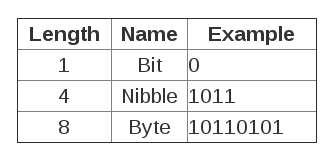
\includegraphics[scale=.6]{content/chapter2/images/bit.png}
	\end{figure}
	
	\end{itemize}
	
\end{flushleft}

\newpage

